\chapter{Execuções para a variação de $E_L$ em torno de $E_0$}

\begin{figure}[phtb]
	\centering
  \begin{tabular}{@{}cc@{}}
    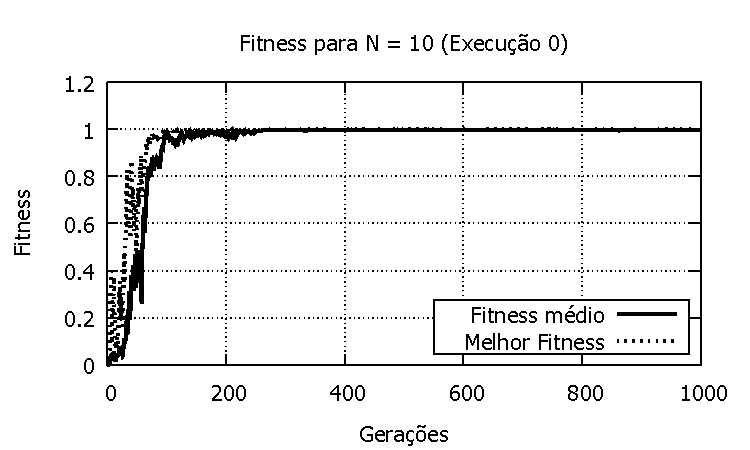
\includegraphics[width=.40\textwidth]{figs/resultados/fitnessEL/N-10_E-0_fitness-extendido.pdf} &
    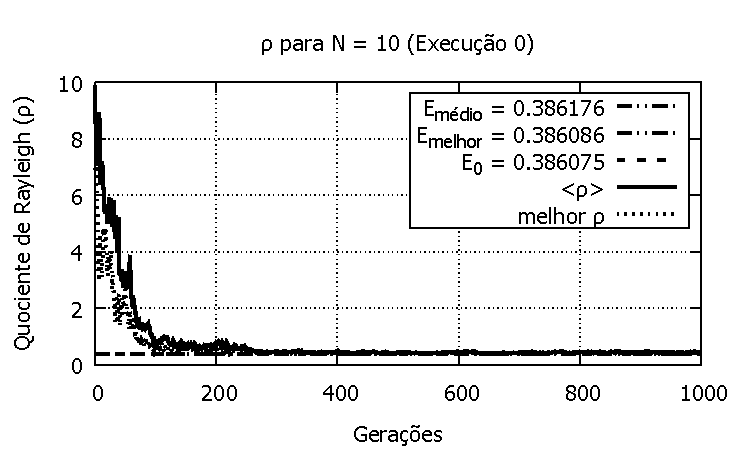
\includegraphics[width=.40\textwidth]{figs/resultados/fitnessEL/N-10_E-0_rho_extendido.pdf}   \\
		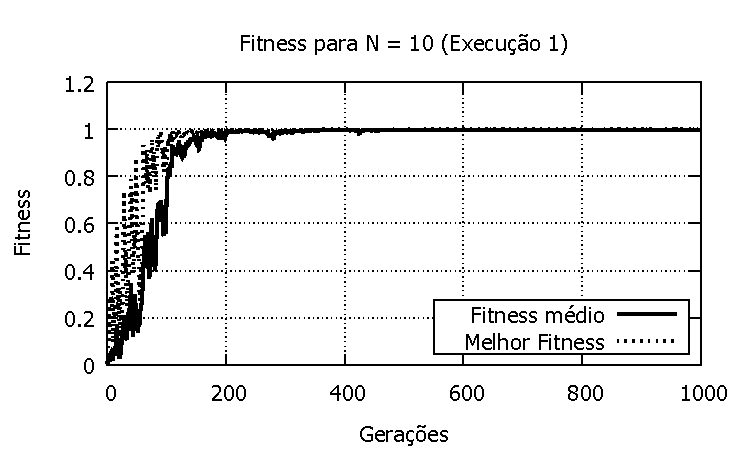
\includegraphics[width=.40\textwidth]{figs/resultados/fitnessEL/N-10_E-1_fitness-extendido.pdf} &
    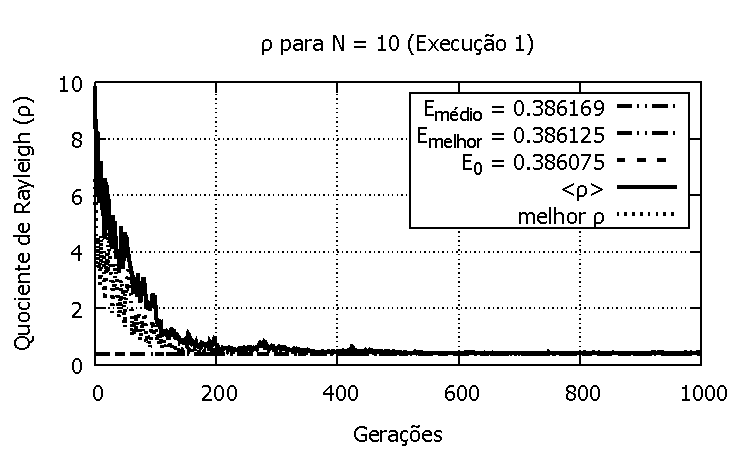
\includegraphics[width=.40\textwidth]{figs/resultados/fitnessEL/N-10_E-1_rho_extendido.pdf}   \\
		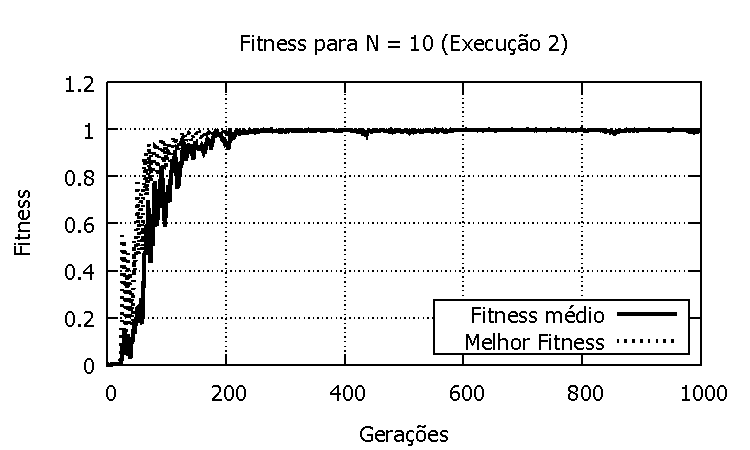
\includegraphics[width=.40\textwidth]{figs/resultados/fitnessEL/N-10_E-2_fitness-extendido.pdf} &
    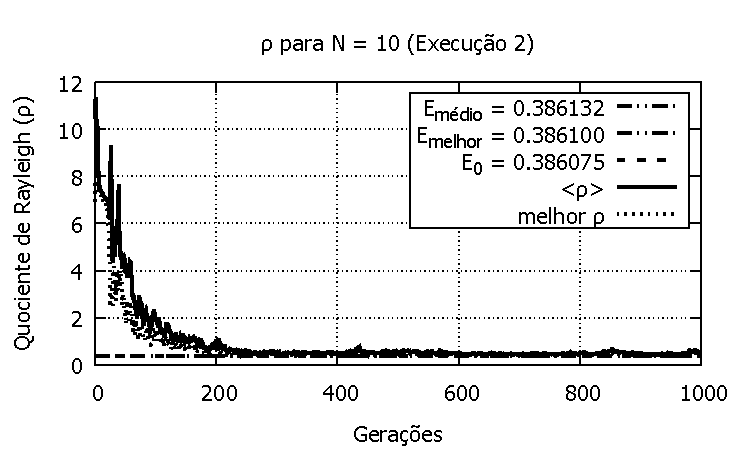
\includegraphics[width=.40\textwidth]{figs/resultados/fitnessEL/N-10_E-2_rho_extendido.pdf}   \\
		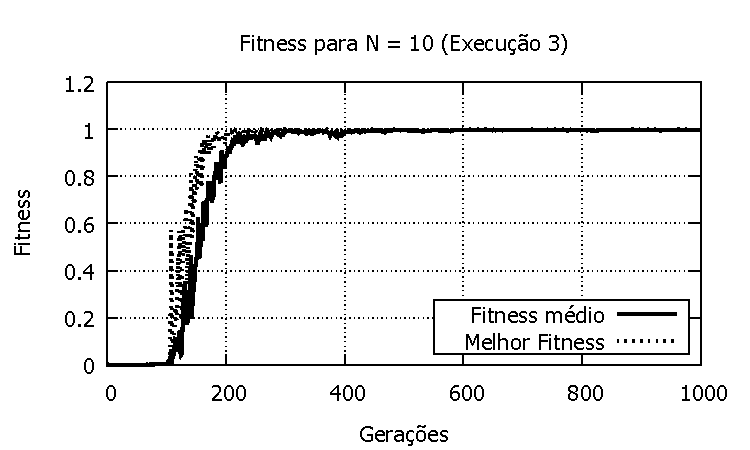
\includegraphics[width=.40\textwidth]{figs/resultados/fitnessEL/N-10_E-3_fitness-extendido.pdf} &
    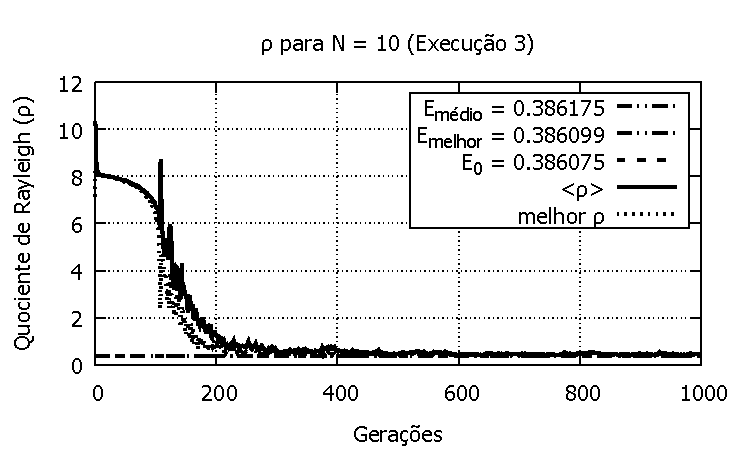
\includegraphics[width=.40\textwidth]{figs/resultados/fitnessEL/N-10_E-3_rho_extendido.pdf}   \\
		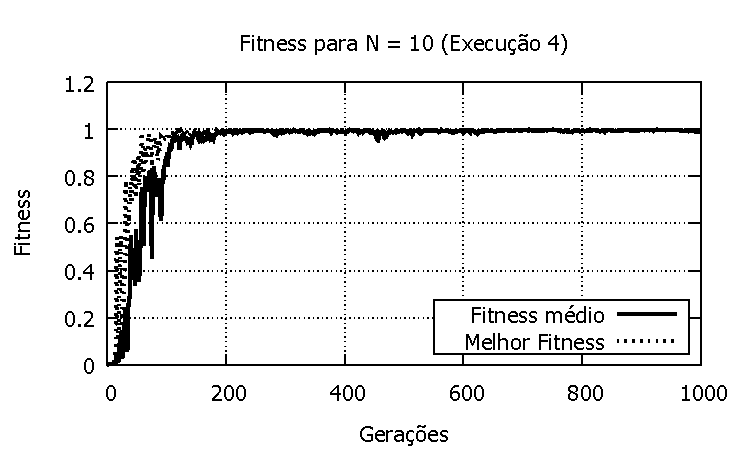
\includegraphics[width=.40\textwidth]{figs/resultados/fitnessEL/N-10_E-4_fitness-extendido.pdf} &
    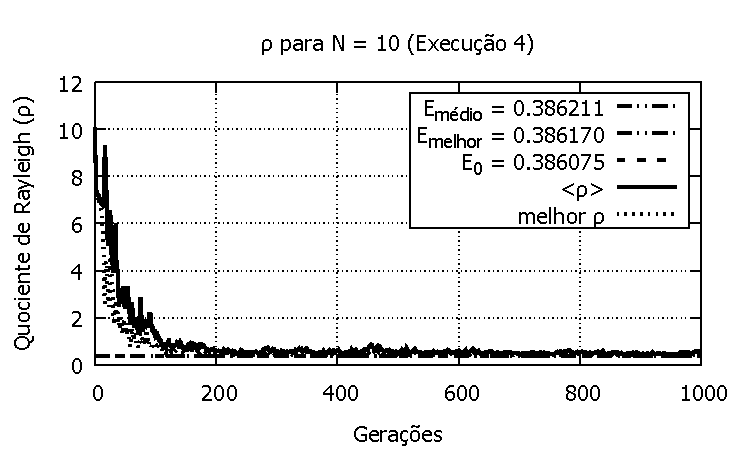
\includegraphics[width=.40\textwidth]{figs/resultados/fitnessEL/N-10_E-4_rho_extendido.pdf} \\
		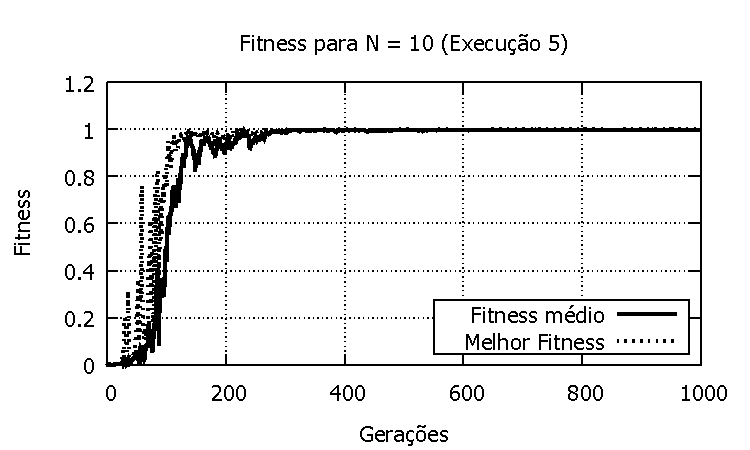
\includegraphics[width=.40\textwidth]{figs/resultados/fitnessEL/N-10_E-5_fitness-extendido.pdf} &
    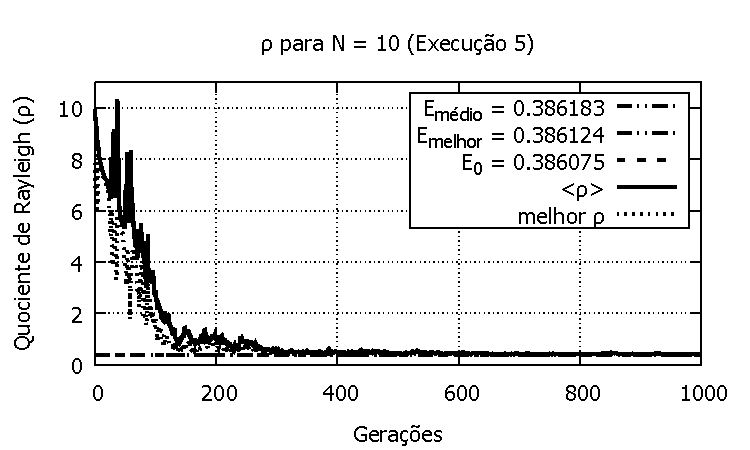
\includegraphics[width=.40\textwidth]{figs/resultados/fitnessEL/N-10_E-5_rho_extendido.pdf}
  \end{tabular}
  \caption{Execuções para N = 10 com o \textit{fitness} $f_i = e^{-\lambda(\rho_i - E_L)^2}$.}
	\label{fig:execucoes_N10_EL}
	\end{figure}
	
	\begin{figure}[phtb]
	\centering
  \begin{tabular}{@{}cc@{}}
		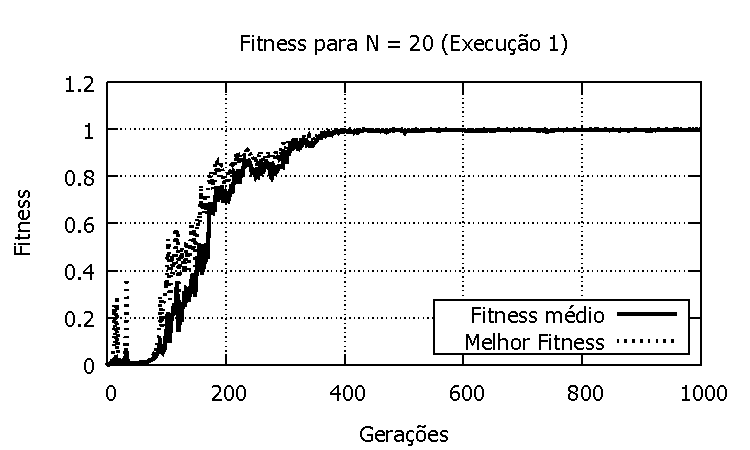
\includegraphics[width=.40\textwidth]{figs/resultados/fitnessEL/N-20_E-1_fitness-extendido.pdf} &
    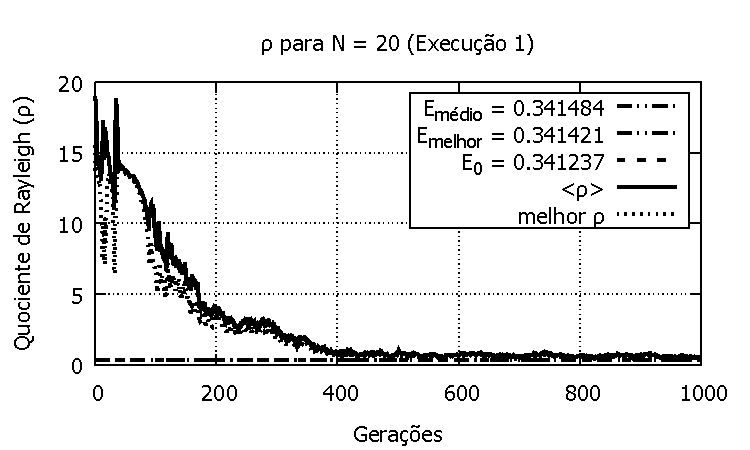
\includegraphics[width=.40\textwidth]{figs/resultados/fitnessEL/N-20_E-1_rho_extendido.pdf}   \\
		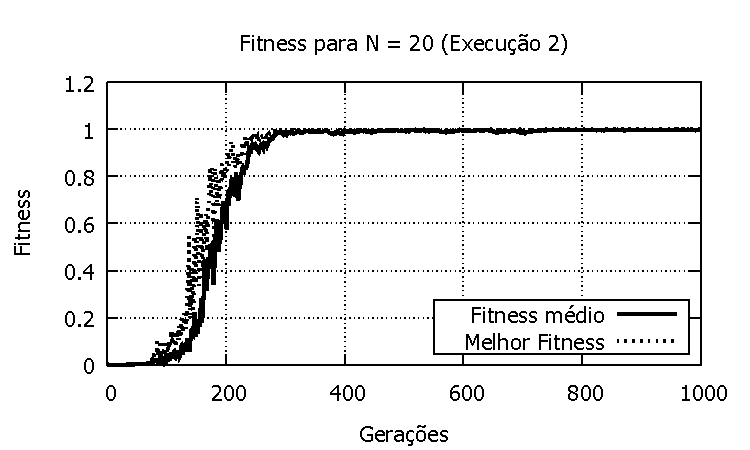
\includegraphics[width=.40\textwidth]{figs/resultados/fitnessEL/N-20_E-2_fitness-extendido.pdf} &
    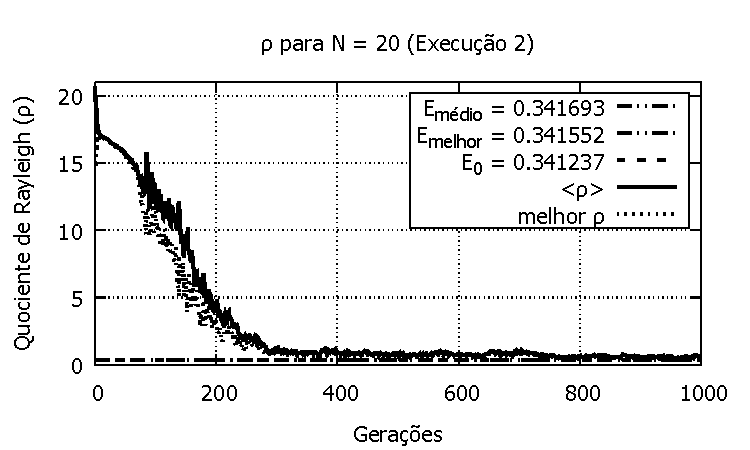
\includegraphics[width=.40\textwidth]{figs/resultados/fitnessEL/N-20_E-2_rho_extendido.pdf}   \\
		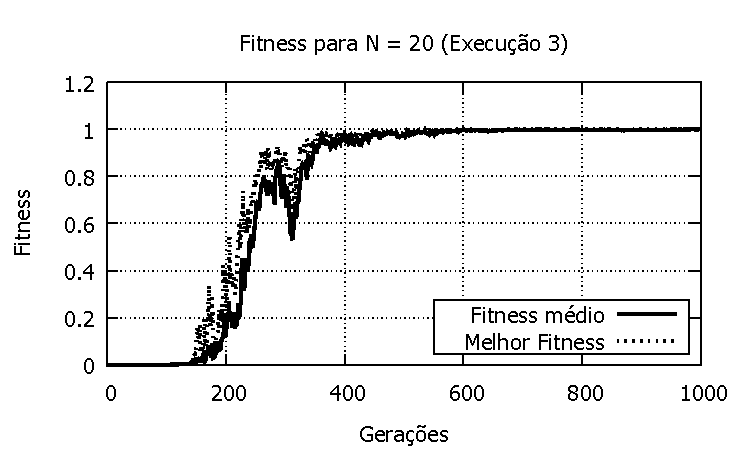
\includegraphics[width=.40\textwidth]{figs/resultados/fitnessEL/N-20_E-3_fitness-extendido.pdf} &
    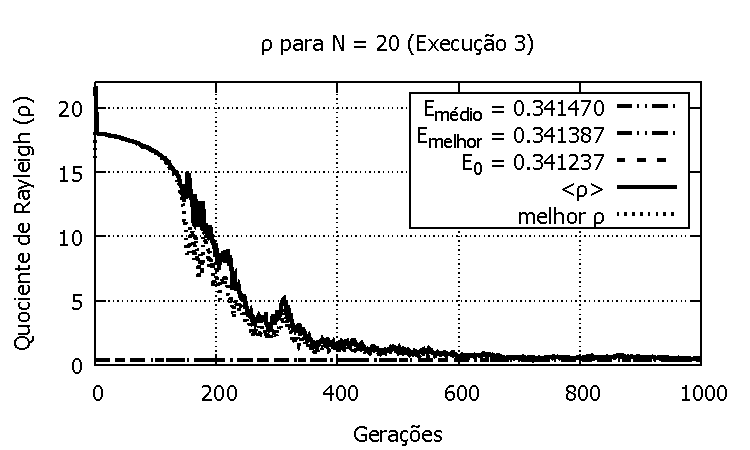
\includegraphics[width=.40\textwidth]{figs/resultados/fitnessEL/N-20_E-3_rho_extendido.pdf}   \\
		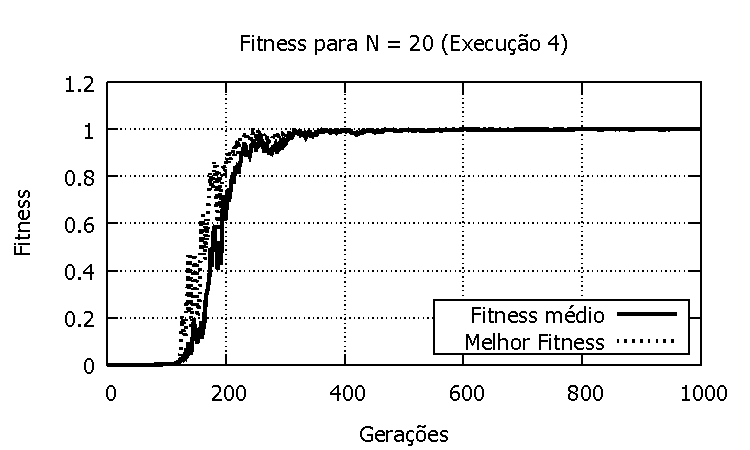
\includegraphics[width=.40\textwidth]{figs/resultados/fitnessEL/N-20_E-4_fitness-extendido.pdf} &
    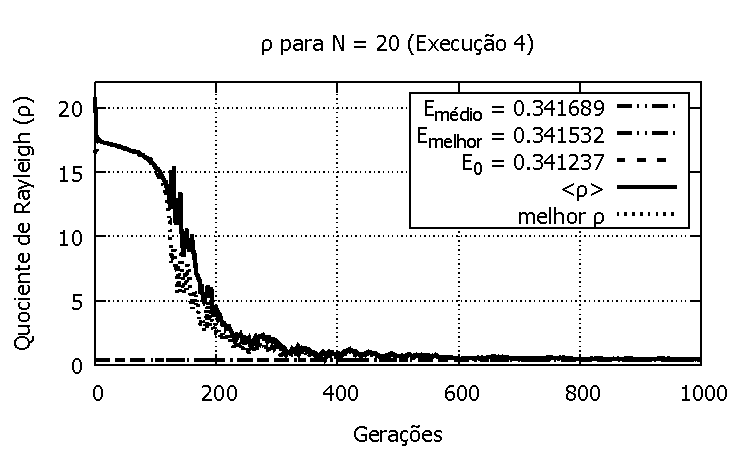
\includegraphics[width=.40\textwidth]{figs/resultados/fitnessEL/N-20_E-4_rho_extendido.pdf} \\
		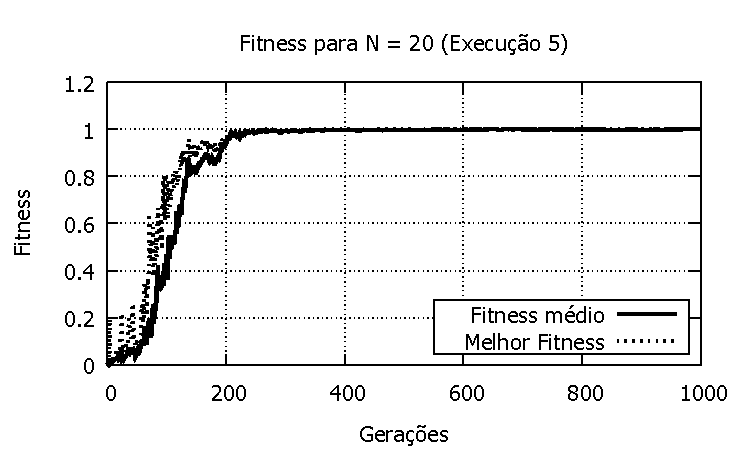
\includegraphics[width=.40\textwidth]{figs/resultados/fitnessEL/N-20_E-5_fitness-extendido.pdf} &
    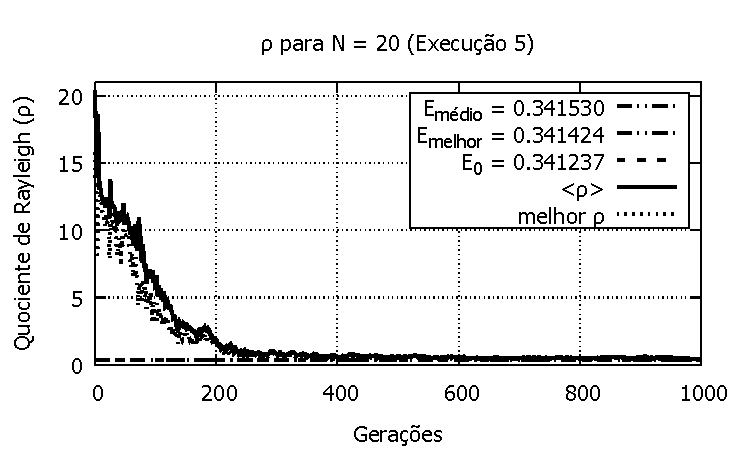
\includegraphics[width=.40\textwidth]{figs/resultados/fitnessEL/N-20_E-5_rho_extendido.pdf}
  \end{tabular}
  \caption{Execuções para N = 20 com o \textit{fitness} $f_i = e^{-\lambda(\rho_i - E_L)^2}$.}
	\label{fig:execucoes_N20_EL}
	\end{figure}
	
	\begin{figure}[phtb]
	\centering
  \begin{tabular}{@{}cc@{}}
		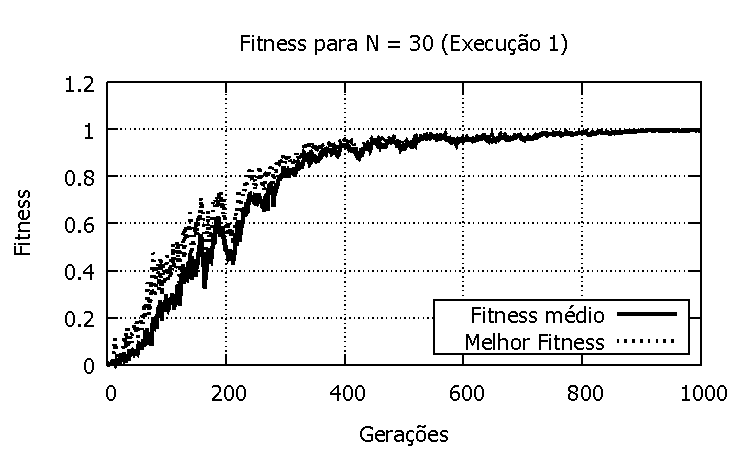
\includegraphics[width=.40\textwidth]{figs/resultados/fitnessEL/N-30_E-1_fitness-extendido.pdf} &
    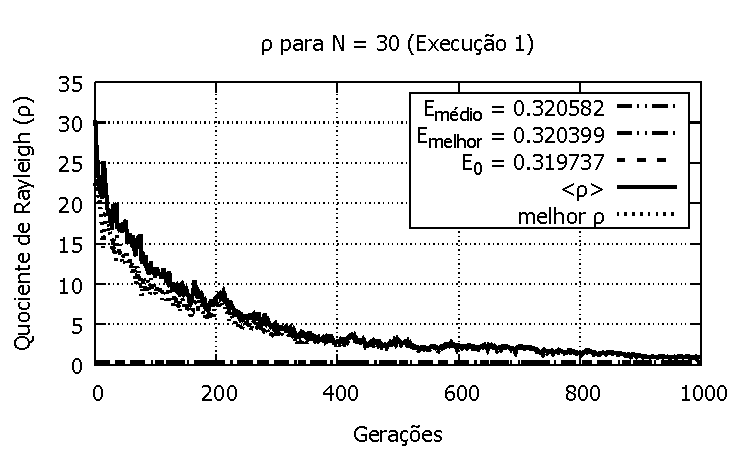
\includegraphics[width=.40\textwidth]{figs/resultados/fitnessEL/N-30_E-1_rho_extendido.pdf}   \\
		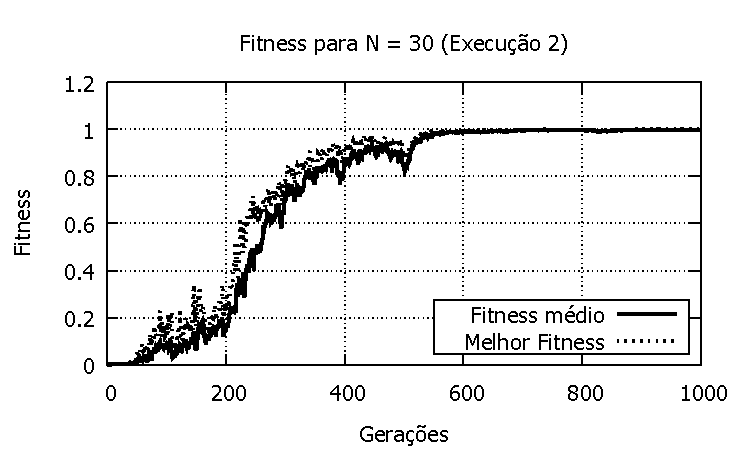
\includegraphics[width=.40\textwidth]{figs/resultados/fitnessEL/N-30_E-2_fitness-extendido.pdf} &
    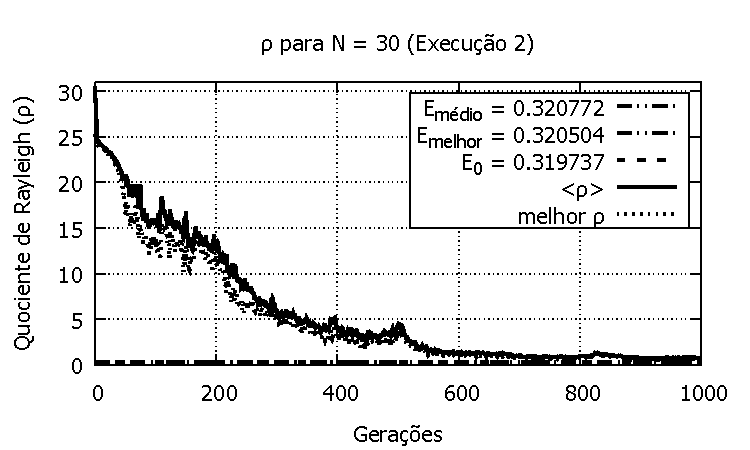
\includegraphics[width=.40\textwidth]{figs/resultados/fitnessEL/N-30_E-2_rho_extendido.pdf}   \\
		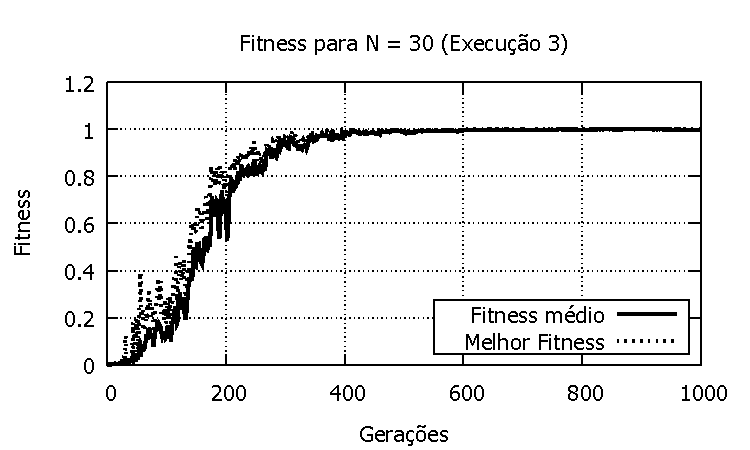
\includegraphics[width=.40\textwidth]{figs/resultados/fitnessEL/N-30_E-3_fitness-extendido.pdf} &
    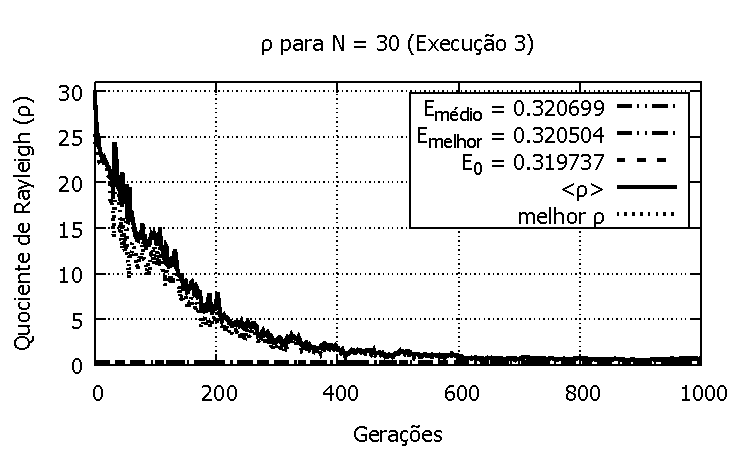
\includegraphics[width=.40\textwidth]{figs/resultados/fitnessEL/N-30_E-3_rho_extendido.pdf}   \\
		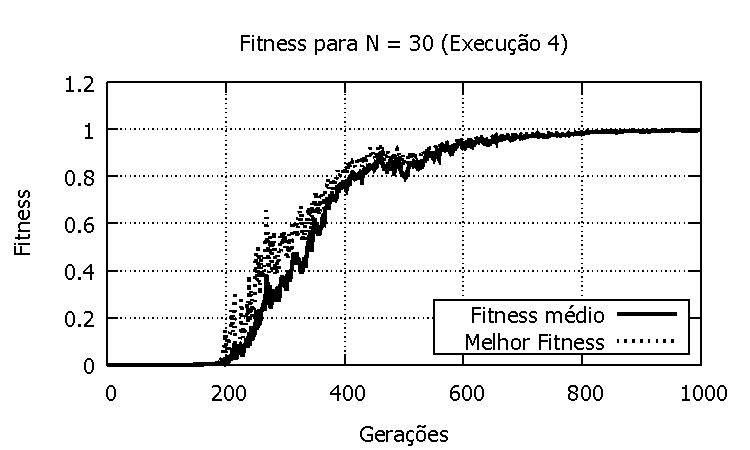
\includegraphics[width=.40\textwidth]{figs/resultados/fitnessEL/N-30_E-4_fitness-extendido.pdf} &
    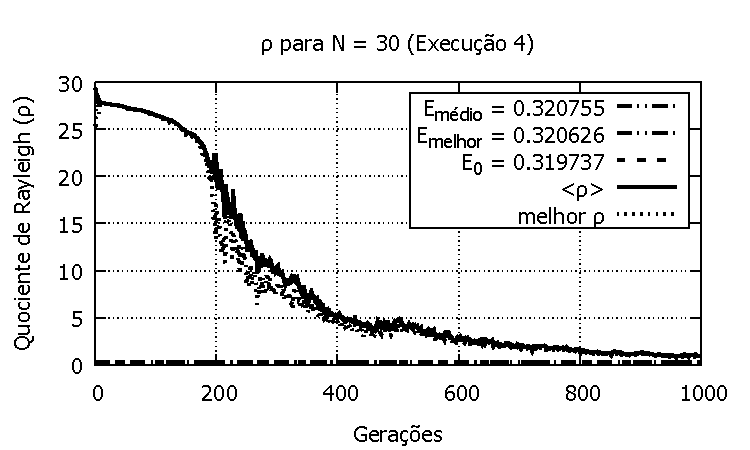
\includegraphics[width=.40\textwidth]{figs/resultados/fitnessEL/N-30_E-4_rho_extendido.pdf} \\
		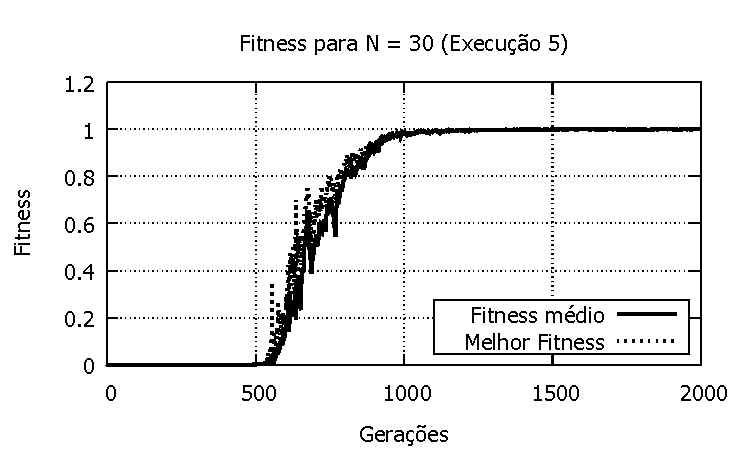
\includegraphics[width=.40\textwidth]{figs/resultados/fitnessEL/N-30_E-5_fitness-extendido.pdf} &
    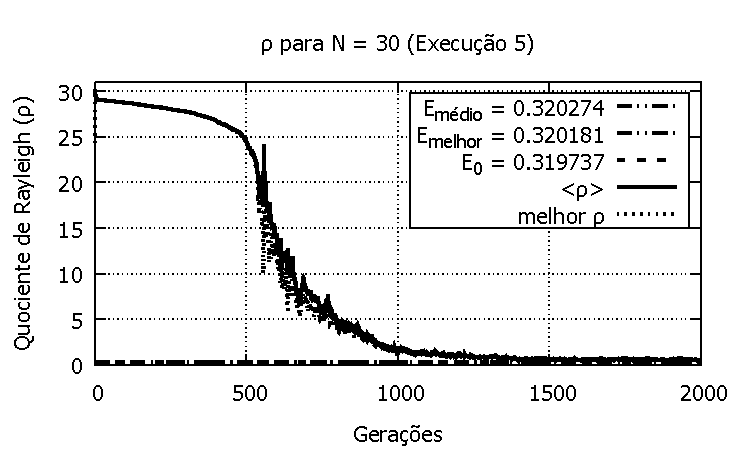
\includegraphics[width=.40\textwidth]{figs/resultados/fitnessEL/N-30_E-5_rho_extendido.pdf}
  \end{tabular}
  \caption{Execuções para N = 30 com o \textit{fitness} $f_i = e^{-\lambda(\rho_i - E_L)^2}$.}
	\label{fig:execucoes_N30_EL}
	\end{figure}
	
	\begin{figure}[phtb]
	\centering
  \begin{tabular}{@{}cc@{}}
		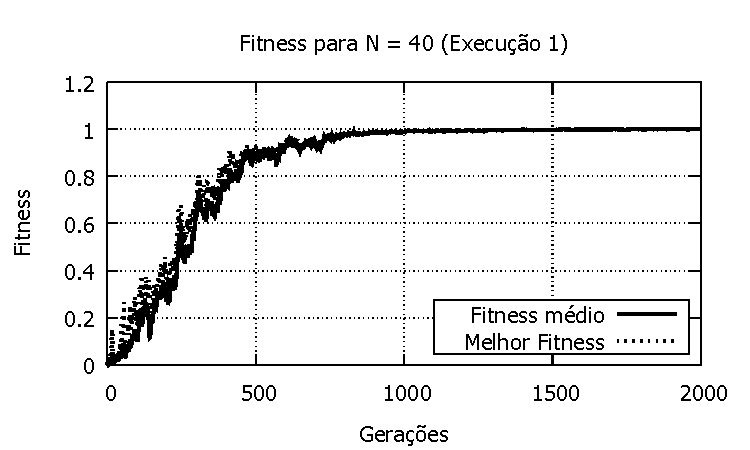
\includegraphics[width=.40\textwidth]{figs/resultados/fitnessEL/N-40_E-1_fitness-extendido.pdf} &
    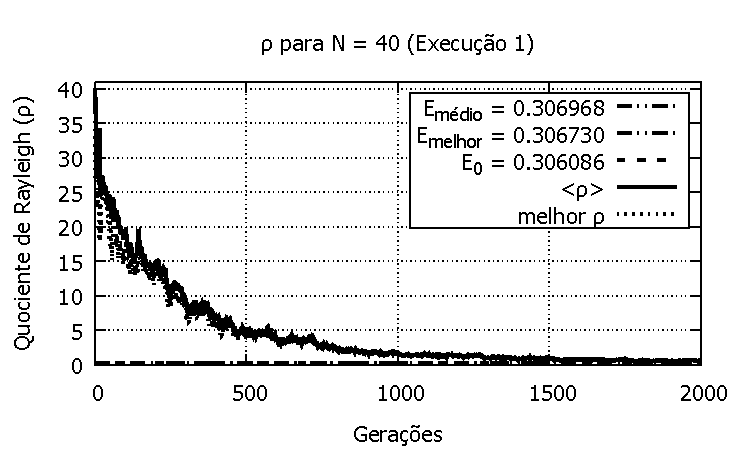
\includegraphics[width=.40\textwidth]{figs/resultados/fitnessEL/N-40_E-1_rho_extendido.pdf}   \\
		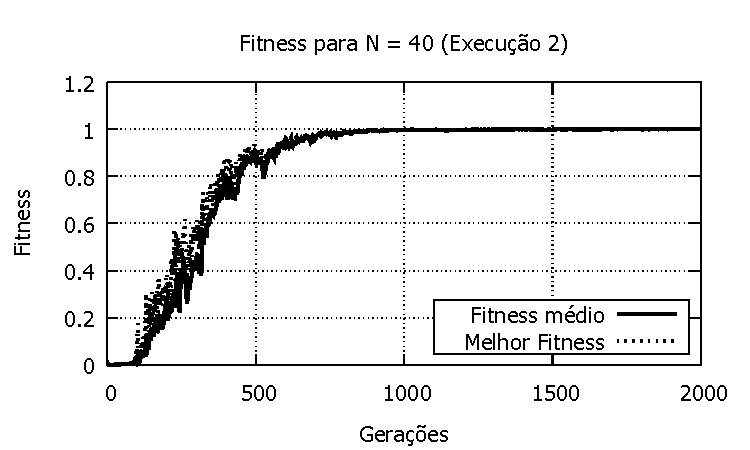
\includegraphics[width=.40\textwidth]{figs/resultados/fitnessEL/N-40_E-2_fitness-extendido.pdf} &
    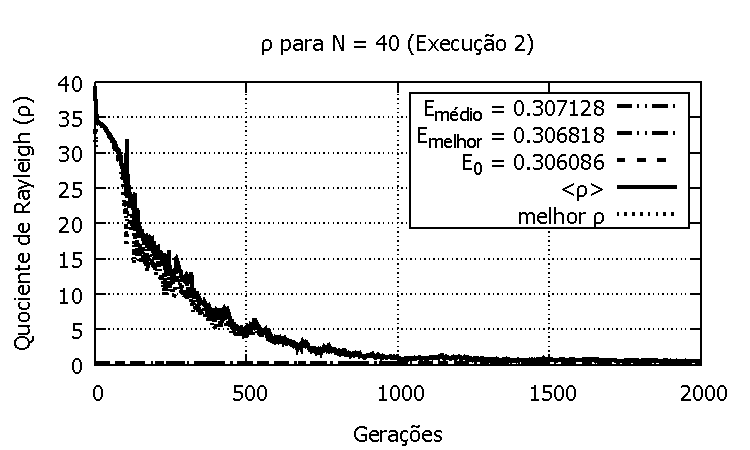
\includegraphics[width=.40\textwidth]{figs/resultados/fitnessEL/N-40_E-2_rho_extendido.pdf}   \\
		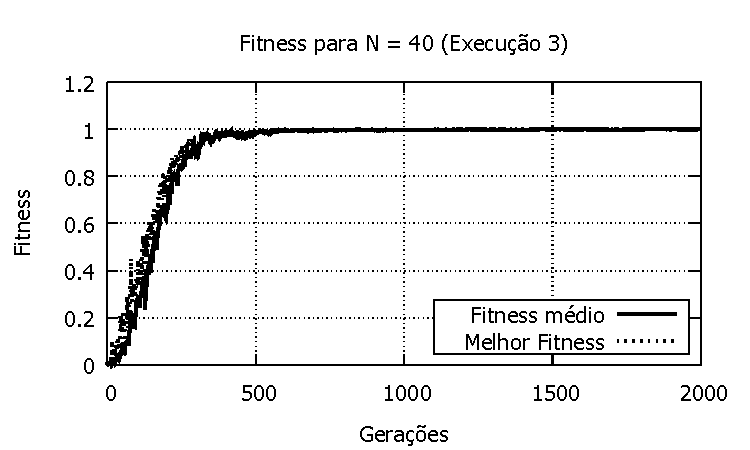
\includegraphics[width=.40\textwidth]{figs/resultados/fitnessEL/N-40_E-3_fitness-extendido.pdf} &
    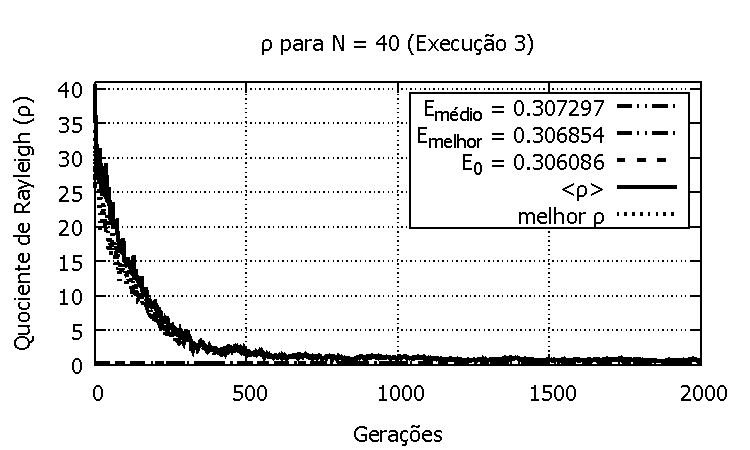
\includegraphics[width=.40\textwidth]{figs/resultados/fitnessEL/N-40_E-3_rho_extendido.pdf}   \\
		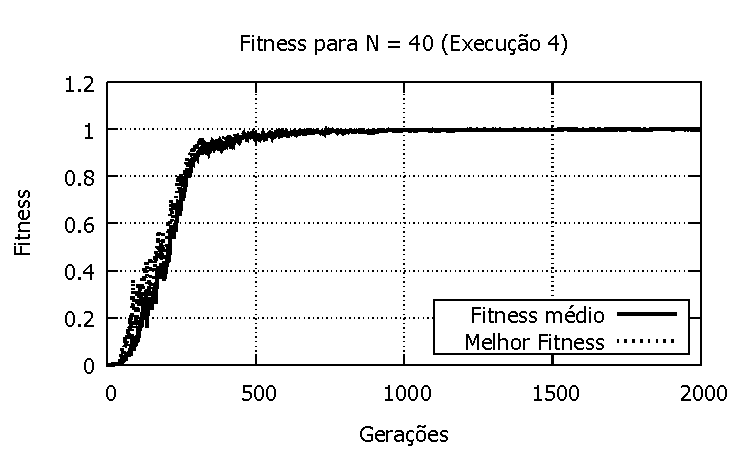
\includegraphics[width=.40\textwidth]{figs/resultados/fitnessEL/N-40_E-4_fitness-extendido.pdf} &
    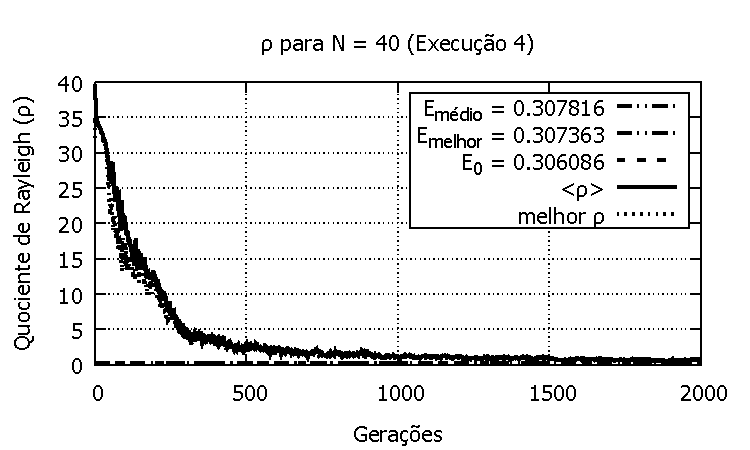
\includegraphics[width=.40\textwidth]{figs/resultados/fitnessEL/N-40_E-4_rho_extendido.pdf}		\\
		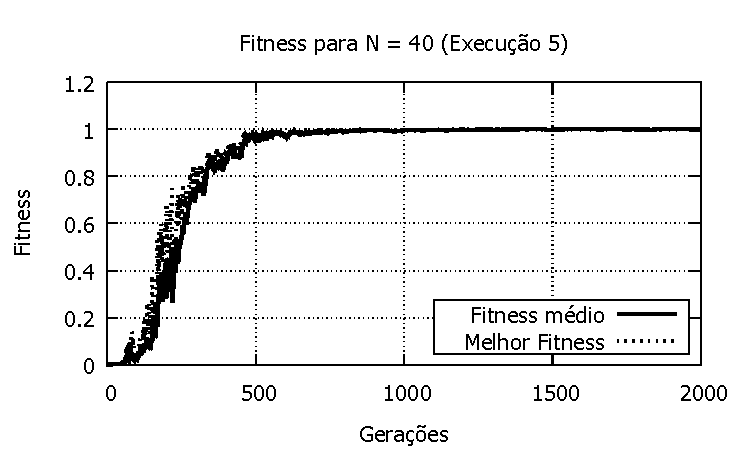
\includegraphics[width=.40\textwidth]{figs/resultados/fitnessEL/N-40_E-5_fitness-extendido.pdf} &
    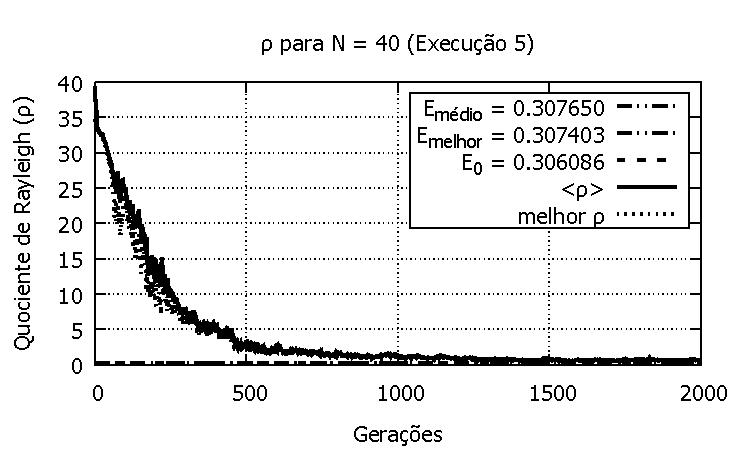
\includegraphics[width=.40\textwidth]{figs/resultados/fitnessEL/N-40_E-5_rho_extendido.pdf}
  \end{tabular}
  \caption{Execuções para N = 40 com o \textit{fitness} $f_i = e^{-\lambda(\rho_i - E_L)^2}$.}
	\label{fig:execucoes_N40_EL}
	\end{figure}